\section{多元函数、极限与连续}
\label{sec:02-Calculus/06-Multivariable-Calculus/01}

单变量微积分里的``连续''，画面上是很清楚的：笔不离开纸，能一笔画出来的曲线就是连续的。而极限呢，无非就是看看从左、右两边走近一个点时，函数值是不是趋于同一个数。这些直觉一旦搬到多元函数的舞台上，原本简单的事情立刻就变得险恶起来。

根源在哪里？一句话：维度升上去了。一维数轴上，你只能向左或向右走；到了二维平面上，四面八方都能走，还可以弯弯绕地走。这就逼着我们必须重新思考，``无限靠近''究竟意味着什么。

\subsection{独木桥与大广场}

回想一下，看一元函数 \(f(x)\) 在 \(x\to a\) 时的极限，我们做的其实只是一件事：检查从左边走近和从右边走近时，函数值会不会撞在一起。这就像在一条独木桥上走向一个点，你只需要看左右两边就够了。

到了二元函数 \(f(x,y)\)，输入空间变成了一片开阔的平面。这时候我们要问的是：当一个动点 \((x,y)\) 无限靠近某个定点 \((x_0,y_0)\) 时，\(f(x,y)\) 的值会怎样？  
问题来了：走近 \((x_0,y_0)\) 的方式一下变得多得不可思议——这里不再是独木桥，而是一个大广场：

\begin{itemize}
    \item 你可以规规矩矩地沿着 \(x\) 轴水平走过去；
    \item 也可以沿着 \(y\) 轴竖直走过去；
    \item 还可以沿着 \(y-y_0 = k(x-x_0)\) 这样任意斜率的直线走过去；
    \item 更可以沿着抛物线 \(x = y^2\) 或者螺旋线，弯弯曲曲地绕进去。
\end{itemize}

这种``走近方式的爆炸''，直接导致了一个要求苛刻的结论：极限要存在，必须保证在所有可能的走近方式下，函数值都趋于同一个数。只要你能找出两条路径，让它们的极限值不一样，或者某条路径根本没有极限，那这个极限就不存在。

这个听起来有点不讲道理的要求，恰恰是多元极限最核心的特征。而要把这层意思说清楚、说严格，最终我们需要一个统一的语言——``距离''，用它来一网打尽所有路径。不过在引出那个形式化的定义之前，我们先用两个经典的反例，把直觉彻底打碎一次。

\subsection{折扇一样的函数：不同方向，不同归宿}

第一个函数是
\[
u(x,y)=\frac{xy}{x^2+y^2},\qquad (x,y)\neq(0,0).
\]
它在原点没定义，分母为零。我们自然会问：能不能在原点给它补一个值，让它连续？也就是说，极限 \(\displaystyle\lim_{(x,y)\to(0,0)}u(x,y)\) 存在吗？如果存在，等于多少？

先学一元的做法，试试最简单的路径——坐标轴：
\begin{itemize}
    \item 沿 \(x\) 轴走（令 \(y=0\)）：对所有 \(x\neq0\)，\(u(x,0)=\frac{0}{x^2}=0\)，极限是 \(0\)；
    \item 沿 \(y\) 轴走（令 \(x=0\)）：对所有 \(y\neq0\)，\(u(0,y)=\frac{0}{y^2}=0\)，极限也是 \(0\)。
\end{itemize}
东西和南北两个方向很一致，似乎补 \(0\) 是理所当然的答案。

但别急，我们换一条斜线试试。沿着过原点的直线 \(y=kx\)（\(k\neq0\)）走进去：
\[
u(x,kx)=\frac{x(kx)}{x^2+(kx)^2}=\frac{kx^2}{(1+k^2)x^2}=\frac{k}{1+k^2}\quad (x\neq0).
\]
值得注意的是，这个表达式里根本没有 \(x\)。也就是说，只要选定了斜率 \(k\)，无论你走到离原点多近的地方，函数值都钉在 \(\frac{k}{1+k^2}\) 这个常数上，保持着这个值一路逼近原点（见下图）：
\begin{itemize}
    \item 沿 \(y=x\)（\(k=1\)），永远是 \(1/2\)；
    \item 沿 \(y=-x\)（\(k=-1\)），永远是 \(-1/2\)；
    \item 沿 \(y=2x\)（\(k=2\)），永远是 \(2/5\)。
\end{itemize}
斜率 \(k\) 一换，常数就跟着变，而且 \(\frac{k}{1+k^2}\) 可以扫出区间 \([-\frac12,\frac12]\) 里的所有值。这意味着从不同角度走近原点，脚下踩着的高度完全不同，函数就像一把从原点撑开的折扇。既然不同的路径给出了不同的极限，那整个极限当然不可能存在。

\begin{center}
\begin{tikzpicture}[x=1cm,y=1cm,font=\small,>=stealth]
  \draw[black!30,dashed] (0,0) circle (2.4);
  \draw[->,black!45] (-2.9,0) -- (2.9,0) node[right] {\(x\)};
  \draw[->,black!45] (0,-2.4) -- (0,2.4) node[above] {\(y\)};
  \draw[blue!70!black,thick] (0,0) -- (2.75,0);
  \draw[blue!70!black,thick] (0,0) -- (1.95,1.95);
  \draw[blue!70!black,thick] (0,0) -- (1.15,2.30);
  \draw[blue!70!black,thick] (0,0) -- (1.95,-1.95);
  \node[right] at (2.8,-0.25) {\(u\equiv 0\)};
  \node[right] at (2.0,1.95) {\(u\equiv \tfrac12\)};
  \node[right] at (1.2,2.35) {\(u\equiv \tfrac25\)};
  \node[right] at (2.0,-1.95) {\(u\equiv -\tfrac12\)};
  \fill (0,0) circle (2pt);
  \draw[<->,black!55] (0,0) -- (-1.70,1.70);
  \node[black!60,above left] at (-0.85,0.85) {\(\delta\)};
\end{tikzpicture}

\emph{沿不同射线走近原点时，函数 \(u(x,y)=xy/(x^2+y^2)\) 恒取不同的常数值，极限不可能存在。}
\end{center}

这个例子告诉我们：在高维空间里，沿着几条直线检查是远远不够的。

\subsection{所有直线都``合格''，照样藏有裂缝}

你也许会想：那我把所有可能的直线方向都查一遍，如果它们全都给出同一个极限，总该没事了吧？

很遗憾，高维世界依然能``暗算''你。来看第二个函数：
\[
f(x,y)=\frac{xy^2}{x^2+y^4},\qquad (x,y)\neq(0,0),
\]
并补充定义 \(f(0,0)=0\)。我们看看它是不是在原点连续。

先试试所有过原点的直线 \(y=kx\)：
\[
f(x,kx)=\frac{x(kx)^2}{x^2+(kx)^4}=\frac{k^2 x^3}{x^2+k^4x^4}=\frac{k^2 x}{1+k^4x^2}\xrightarrow{x\to 0} 0.
\]
沿 \(x=0\)（也就是 \(y\) 轴），\(f(0,y)=0\)，同样趋于 \(0\)。  
你看，不论直线是平是陡，极限清一色全是 \(0\)。如果还用一元的直觉，你大概已经认定极限是 \(0\)，函数连续了。

但这次我们故意走一条弯的路线——沿抛物线 \(x = y^2\) 走进去：
\[
f(y^2,y)=\frac{(y^2)\cdot y^2}{(y^2)^2+y^4}=\frac{y^4}{2y^4}=\frac{1}{2}\quad (y\neq0).
\]
函数值居然稳稳地停在 \(1/2\)，完全不趋于 \(0\)！

这里发生了什么？打个比方：所有的直线都因为``太直''，恰好跨过了藏在曲面里的一条抛物线裂缝；只有当你弯下身子、顺着抛物线走进去时，才会一脚踩进这条裂缝里。这个例子无情地告诉我们：\textbf{即使穷尽所有直线，也不足以验证多元函数的极限。}

\subsection{破局的办法：忘掉方向，只看距离}即使穷尽所有直线，也不足以验证多元函数的极限。

从上面两个反例里，我们能总结出两件事：
\begin{enumerate}
    \item 要证明极限不存在，往往不算太难：只要你能挑出两条路径，让它们给出不同的极限（或者某条路径压根儿没有极限），结论就板上钉钉了。
    \item 但要证明极限存在，可就严苛多了——你必须一次性按住所有可能的路径，直线的、弯曲的、螺旋的，一条都不能漏。
\end{enumerate}

那数学上怎么才能做到``一次性按住所有路径''呢？办法说起来也简单：别管路径怎么弯，只盯住它到目标点的距离。

\subsection{\texorpdfstring{\(\varepsilon\)-\(\delta\)}{ε-δ} 定义：用小圆盘罩住所有路径}

回想一下一元函数极限的 \(\varepsilon\)-\(\delta\) 定义：
\[
\lim_{x\to a}f(x)=L \iff \forall\varepsilon>0,\;\exists\delta>0,\; \text{当 }0<|x-a|<\delta \text{ 时},\; |f(x)-L|<\varepsilon.
\]
这里 \(|x-a|\) 就是数轴上点 \(x\) 到 \(a\) 的距离。只要距离够小，函数值就够接近 \(L\)。

平面上，点 \((x,y)\) 到 \((x_0,y_0)\) 的距离自然取欧氏距离
\[
r=\sqrt{(x-x_0)^2+(y-y_0)^2}.
\]
一个以 \((x_0,y_0)\) 为圆心、\(\delta\) 为半径的小圆盘，就把从所有可能方向、沿所有可能路径无限逼近这个点的全部情况都包含在里面了（见下图）。不管路径多曲折，只要它最终钻进这个圆盘，它上面每一个点都满足 \(r<\delta\)。

\begin{center}
\begin{tikzpicture}[scale=1.2]
  \draw[->] (-1,0) -- (4,0) node[right] {\(x\)};
  \draw[->] (0,-1) -- (0,3) node[above] {\(y\)};
    \filldraw (2,1.5) circle (1.5pt) node[below left] {\((x_0,y_0)\)};
  \draw[dashed] (2,1.5) circle (1.2);
    \draw[<->] (2,1.5) -- ++(0.8485,0.8485) node[midway,above left] {\(\delta\)};
    \node[fill=white,inner sep=1pt] at (2.75,1.75) {\(0<r<\delta\)};
\end{tikzpicture}

\emph{以 \((x_0,y_0)\) 为心、\(\delta\) 为半径的圆盘，囊括了所有逼近路径，不再需要单独关心方向。}
\end{center}

这就直接引出了二元函数极限的正式定义：

\begin{definition}[二元函数的极限]
设函数 \(f\) 在点 \((x_0,y_0)\) 的某个去心邻域内有定义，\(L\) 为实数。如果对任意给定的 \(\varepsilon>0\)，总能找到 \(\delta>0\)，使得当
\[
0<\sqrt{(x-x_0)^2+(y-y_0)^2}<\delta
\]
时，恒有
\[
|f(x,y)-L|<\varepsilon,
\]
就称当 \((x,y)\) 趋于 \((x_0,y_0)\) 时 \(f(x,y)\) 的极限为 \(L\)，记作
\[
\lim_{(x,y)\to(x_0,y_0)}f(x,y)=L.
\]
\end{definition}

这个定义的精髓在于：它只要求当点落在一个充分小的圆盘里（无论从哪个方向进来的），函数值就与 \(L\) 任意接近。它不给任何特殊路径留作弊的空间。

\subsection{用定义真正证出一个极限}

现在，我们正面试一个``听话''的函数。设
\[
g(x,y)=\frac{x^2y}{x^2+y^2},\qquad (x,y)\neq(0,0),
\]
并补充 \(g(0,0)=0\)。我们猜测 \(\displaystyle\lim_{(x,y)\to(0,0)}g(x,y)=0\)。

怎么证？对任意给定的 \(\varepsilon>0\)，我们要找出一个 \(\delta>0\)，使得只要 \(0<\sqrt{x^2+y^2}<\delta\)，就保证 \(|g(x,y)-0|<\varepsilon\)。

观察一下分子分母的结构。因为 \(x^2\le x^2+y^2\)，所以
\[
\frac{x^2}{x^2+y^2}\le 1
\]
对所有 \((x,y)\neq(0,0)\) 成立。于是
\[
|g(x,y)| = |y|\cdot\frac{x^2}{x^2+y^2} \le |y|.
\]
又因为 \(|y|\le\sqrt{x^2+y^2}\)，我们得到一个漂亮的不等式：
\[
|g(x,y)| \le \sqrt{x^2+y^2}.
\]
这下方向信息完全消失了——函数值的绝对值被纯粹用距离控制住了。既然如此，只需取 \(\delta=\varepsilon\)：当 \(0<\sqrt{x^2+y^2}<\delta\) 时，
\[
|g(x,y)-0| \le \sqrt{x^2+y^2} < \delta = \varepsilon.
\]
恰好满足定义的要求，所以极限就是 \(0\)。证完了。

熟悉极坐标的读者可能会发现，这个问题用极坐标几乎是一眼看穿：令 \(x=r\cos\theta\), \(y=r\sin\theta\)，则
\[
g(r\cos\theta,r\sin\theta)=\frac{r^3\cos^2\theta\sin\theta}{r^2}=r\cos^2\theta\sin\theta.
\]
因为 \(|\cos^2\theta\sin\theta|\le 1\)，所以 \(|g|\le r=\sqrt{x^2+y^2}\)。不论角度 \(\theta\) 怎么变，只要 \(r\to0\)，函数值就被夹逼着趋于 \(0\)。这也再次印证了前面的证明。

不过要提醒一句：极坐标方法成立的前提，是你能把函数绝对值放大成一个只与 \(r\) 有关且趋于 \(0\) 的量。如果上界还跟 \(\theta\) 掰扯不清，那就不能直接下结论。

\subsection{连续性：把极限和函数值对上}

有了极限的严格定义，连续性就水到渠成了。

\begin{definition}[二元函数的连续性]
设函数 \(f\) 在点 \((x_0,y_0)\) 的某邻域内有定义。如果
\[
\lim_{(x,y)\to(x_0,y_0)}f(x,y)=f(x_0,y_0),
\]
则称 \(f\) 在点 \((x_0,y_0)\) 连续。如果 \(f\) 在区域 \(D\) 上每一点都连续，就称它在 \(D\) 上连续。
\end{definition}

对照前面的例子，立刻可以看出：
\begin{itemize}
    \item \(g(x,y)=\frac{x^2y}{x^2+y^2}\) 配上 \(g(0,0)=0\)，在原点连续，因为极限等于 \(0\)，定义值也是 \(0\)。
    \item 第一个反例 \(u(x,y)=\frac{xy}{x^2+y^2}\)，不管你在原点补什么值，都不可能连续——极限根本就不存在。
    \item 第二个反例 \(f(x,y)=\frac{xy^2}{x^2+y^4}\)，虽然沿所有直线的极限都是 \(0\)，但它沿抛物线的极限是 \(1/2\)，和定义值 \(f(0,0)=0\) 对不上，所以也不连续。
\end{itemize}

从证明技巧的角度再捋一下：
\begin{itemize}
    \item 证连续（或证极限存在）：必须用 \(\varepsilon\)-\(\delta\) 或极坐标放缩，得出一个仅与距离有关的控制。
    \item 证不连续（极限不存在）：相对简单，找出两条路径导致不同极限即可。经典的``坏路径''包括 \(y=kx\)、\(y=x^\alpha\)、\(x=y^2\) 等等。
\end{itemize}

\subsection{这一节留下的教训}

多元函数的极限与连续，给我们的最深一课是：局部方向上的太平，绝不代表整体的太平。

单变量的时候，左右极限一致就万事大吉；到了多元，你面对的是一个无穷无尽的方向集合，抽查若干条甚至无穷多条直线，都不足以让你高枕无忧。唯有抓住``距离''这个概念，用一个统一的小圆盘把所有路径全部罩住，才能真正驯服极限。

这个思想会一路贯穿整个多元微积分。接下来的章节里你会看到，类似的陷阱又一次上演：一个函数即使沿各个坐标轴方向的偏导数都完美存在，它在局部也未必真的``光滑''——可能根本不存在一个像样的切平面。到那时，我们仍然要拿起``距离''和``线性近似误差''这两样工具，去分辨谁是真的可微，谁只是假象。